\documentclass[journal]{vgtc}                % final (journal style)
%\documentclass[review,journal]{vgtc}         % review (journal style)
%\documentclass[widereview]{vgtc}             % wide-spaced review
%\documentclass[preprint,journal]{vgtc}       % preprint (journal style)

%% Uncomment one of the lines above depending on where your paper is
%% in the conference process. ``review'' and ``widereview'' are for review
%% submission, ``preprint'' is for pre-publication, and the final version
%% doesn't use a specific qualifier.

%% Please use one of the ``review'' options in combination with the
%% assigned online id (see below) ONLY if your paper uses a double blind
%% review process. Some conferences, like IEEE Vis and InfoVis, have NOT
%% in the past.

%% Please note that the use of figures other than the optional teaser is not permitted on the first page
%% of the journal version.  Figures should begin on the second page and be
%% in CMYK or Grey scale format, otherwise, colour shifting may occur
%% during the printing process.  Papers submitted with figures other than the optional teaser on the
%% first page will be refused. Also, the teaser figure should only have the
%% width of the abstract as the template enforces it.

%% These few lines make a distinction between latex and pdflatex calls and they
%% bring in essential packages for graphics and font handling.
%% Note that due to the \DeclareGraphicsExtensions{} call it is no longer necessary
%% to provide the the path and extension of a graphics file:
%% 
\includegraphics{diamondrule} is completely sufficient.
%%
\ifpdf%                                % if we use pdflatex
  \pdfoutput=1\relax                   % create PDFs from pdfLaTeX
  \pdfcompresslevel=9                  % PDF Compression
  \pdfoptionpdfminorversion=7          % create PDF 1.7
  \ExecuteOptions{pdftex}
  \usepackage{graphicx}                % allow us to embed graphics files
  \DeclareGraphicsExtensions{.pdf,.png,.jpg,.jpeg} % for pdflatex we expect .pdf, .png, or .jpg files
\else%                                 % else we use pure latex
  \ExecuteOptions{dvips}
  \usepackage{graphicx}                % allow us to embed graphics files
  \DeclareGraphicsExtensions{.eps}     % for pure latex we expect eps files
\fi%

%% it is recomended to use ``\autoref{sec:bla}'' instead of ``Fig.~\ref{sec:bla}''
\graphicspath{{figures/}{pictures/}{images/}{./}} % where to search for the images

\usepackage{microtype}                 % use micro-typography (slightly more compact, better to read)
\PassOptionsToPackage{warn}{textcomp}  % to address font issues with \textrightarrow
\usepackage{textcomp}                  % use better special symbols
\usepackage{mathptmx}                  % use matching math font
\usepackage{times}                     % we use Times as the main font
\renewcommand*\ttdefault{txtt}         % a nicer typewriter font
\usepackage{cite}                      % needed to automatically sort the references
\usepackage{tabu}                      % only used for the table example
\usepackage{booktabs}                  % only used for the table example
%% We encourage the use of mathptmx for consistent usage of times font
%% throughout the proceedings. However, if you encounter conflicts
%% with other math-related packages, you may want to disable it.

%% In preprint mode you may define your own headline.
%\preprinttext{To appear in IEEE Transactions on Visualization and Computer Graphics.}

%% If you are submitting a paper to a conference for review with a double
%% blind reviewing process, please replace the value ``0'' below with your
%% OnlineID. Otherwise, you may safely leave it at ``0''.
\onlineid{0}

%% declare the category of your paper, only shown in review mode
\vgtccategory{Research}
%% please declare the paper type of your paper to help reviewers, only shown in review mode
%% choices:
%% * algorithm/technique
%% * application/design study
%% * evaluation
%% * system
%% * theory/model
\vgtcpapertype{please specify}

%% Paper title.
\title{Data Comets}

%% This is how authors are specified in the journal style

%% indicate IEEE Member or Student Member in form indicated below
\author{Aristotelis Sigiouan Leventidis, Berk Can Gurel, David Saffo, Twinke Jain}
\authorfooter{
%% insert punctuation at end of each item
\item
 Aristotelis Sigiouan Leventidis, Northeastern University, Email: leventidis.a@husky.neu.edu
\item
 Berk Can Gurel, Northeastern University, Email: gurel.b@husky.neu.edu
\item
 David Saffo, Northeastern University, Email: saffo.d@husky.neu.edu
 \item
 Twinkle Jain, Northeastern University, Email: jain.t@husky.neu.edu
}

%other entries to be set up for journal
\shortauthortitle{Biv \MakeLowercase{\textit{et al.}}: Global Illumination for Fun and Profit}
%\shortauthortitle{Firstauthor \MakeLowercase{\textit{et al.}}: Paper Title}

%% Abstract section.
\abstract{ Abstract
} % end of abstract

%% Keywords that describe your work. Will show as 'Index Terms' in journal
%% please capitalize first letter and insert punctuation after last keyword
\keywords{Drone, d3, map overlay}

%% ACM Computing Classification System (CCS). 
%% See <http://www.acm.org/class/1998/> for details.
%% The ``\CCScat'' command takes four arguments.

\CCScatlist{ % not used in journal version
 \CCScat{K.6.1}{Management of Computing and Information Systems}%
{Project and People Management}{Life Cycle};
 \CCScat{K.7.m}{The Computing Profession}{Miscellaneous}{Ethics}
}

%% Uncomment below to include a teaser figure.
\teaser{
  \centering
  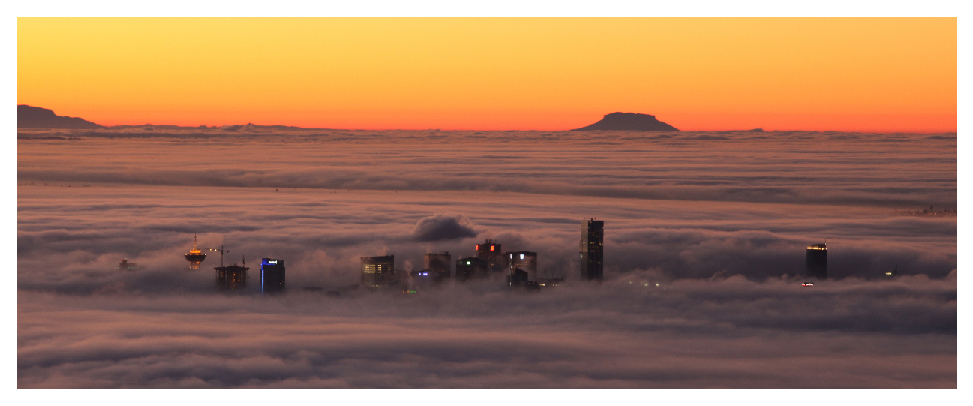
\includegraphics[width=\linewidth]{CypressView}
  \caption{Data Comets visualization}
	\label{fig:teaser}
}

%% Uncomment below to disable the manuscript note
\renewcommand{\manuscriptnotetxt}{}

%% Copyright space is enabled by default as required by guidelines.
%% It is disabled by the 'review' option or via the following command:
% \nocopyrightspace

\vgtcinsertpkg

%%%%%%%%%%%%%%%%%%%%%%%%%%%%%%%%%%%%%%%%%%%%%%%%%%%%%%%%%%%%%%%%
%%%%%%%%%%%%%%%%%%%%%% START OF THE PAPER %%%%%%%%%%%%%%%%%%%%%%
%%%%%%%%%%%%%%%%%%%%%%%%%%%%%%%%%%%%%%%%%%%%%%%%%%%%%%%%%%%%%%%%%

\begin{document}

%% The ``\maketitle'' command must be the first command after the
%% ``\begin{document}'' command. It prepares and prints the title block.

%% the only exception to this rule is the \firstsection command
\firstsection{Introduction}

\maketitle

%% \section{Introduction} %for journal use above \firstsection{..} instead
Brief introduction to our project and a short explanation of the paper sections.

\section{Related Work}

In this section we will talk about previous work done about drone or object trajectories. We will discuss how those papers or projects are relevant to our work and what are their limitations.

\section{Process}

In this section we will explain our implementation process in subsections.

	\subsection{Dataset}
	
	We will talk about the dataset we use for this project. What is the source of the data? How many examples and dimension are there? How complete is the data? Is the dataset reliable?
	
	\subsection{Data Filtering and Preprocessing}
	
	We will describe the operations we apply to the raw data in order to get preprocessed data.
	
	\subsection{Map Embeddings}
	
	How do we retrieve the map and how do we embed it to the background? Is the map interactive?
	
	\subsection{Visualizing Trajectories}
	
	We will describe our algorithms to visualize the drone trajectories over the map. We will explain how the trajectories and the trails are calculated and plotted.
	
	\subsection{Plotting Charts and Graphs}
	
	We will talk about how to plot the charts and graphs for our interface.
	
	\subsection{Brushing and Linking}
	
	How interactive the visualization is? How can we make selections? Which components are linked? How the linking is achieved?

\section{Design}

In this section we will explain our design choices in subsections.

	\subsection{Encodings}
	
	How many attributes are encoded? Which marks and channels did we use and why?
	
	\subsection{Color and Shape Choices}
	
	How did we choose which color scales to use and why? How did we decide on the shape and size of the trajectory and the trail?
	
	\subsection{Data\&Ink Redundancy}
	
	What did we do to ensure that our visualization is easy to read and understand?

\section{Discussion}

In this section we will talk about our results and what we have achieved.

	\subsection{Challenges and Limitations}
	
	Which parts of the projects were challenging for us? Which functions we have failed to implement?
	
	\subsection{Future Work}
	
	What are the plans for the future of this project? What can be further improved?

\section{Conclusion}

In the conclusion, we will give a brief summary of the paper and our findings.

\section{References}



%% if specified like this the section will be committed in review mode
%\acknowledgments{}

%\bibliographystyle{abbrv}
\bibliographystyle{abbrv-doi}
%\bibliographystyle{abbrv-doi-narrow}
%\bibliographystyle{abbrv-doi-hyperref}
%\bibliographystyle{abbrv-doi-hyperref-narrow}

\bibliography{template}
\end{document}

